\documentclass[conference]{IEEEtran}
\usepackage{amsmath}
\usepackage{array}
\usepackage{graphicx}
\usepackage[hidelinks]{hyperref}
\newcommand{\RunDuration}{28.60}
\newcommand{\RunSamples}{573}
\newcommand{\RunRMSE}{0.12}
\newcommand{\RunMax}{0.33}
\newcommand{\RunFinal}{6.60}
\newcommand{\RunProgress}{15.23}

\title{Design and Figure-Eight Tracking of an Ackermann Mobile Robot in ROS 2 and Gazebo}
\author{\IEEEauthorblockN{Robotics Project Group 4}
\IEEEauthorblockA{Ackermann Challenger mobile robotics project}}
\begin{document}
\maketitle

\begin{abstract}
This paper describes the mechanical design, kinematic modeling, and simulation of a rear-driven mobile robot with Ackermann steering. A Fusion 360 assembly was imported into Gazebo Harmonic through a URDF/Xacro description and controlled by a ROS 2 Jazzy Pure Pursuit node. The reference was a 15.29-m figure eight with curvature bounded by the steering design. One Gazebo run using simulated rear-axle pose feedback achieved a root mean square path error of \RunRMSE\ cm and a peak error of \RunMax\ cm. The comparison with differential, skid-steer, and omnidirectional platforms motivates Ackermann steering for continuous forward routes on paved surfaces with adequate turning clearance.
\end{abstract}

\begin{IEEEkeywords}
Ackermann steering, mobile robots, Pure Pursuit, ROS 2, Gazebo, path tracking.
\end{IEEEkeywords}

\section{Introduction}
Wheeled robot architectures differ in their admissible velocities and rolling constraints~\cite{lynch}. The Ackermann Challenger uses rear drive and two front steering joints. The project imports the Fusion 360 geometry into Gazebo and measures closed-loop tracking on a route with turns in both directions and a self-intersection.

\section{Kinematic Comparison}
Table~\ref{tab:comparison} compares differential drive, skid-steer, omnidirectional drive, and a physical single-steer tricycle. The last helps distinguish a physical platform from the virtual bicycle approximation in Section~III. A differential platform with two driven wheels and passive casters can spin without the lateral tire scrub characteristic of fixed four-wheel skid-steer. Real mechanisms and surfaces introduce slip even where an ideal kinematic model predicts rolling.

\begin{table}[t]
\caption{Wheeled Mobility Trade-Offs}
\label{tab:comparison}
\centering\small
\begin{tabular}{@{}>{\raggedright\arraybackslash}p{0.22\columnwidth}
  >{\raggedright\arraybackslash}p{0.30\columnwidth}
  >{\raggedright\arraybackslash}p{0.37\columnwidth}@{}}
\hline
Model & Benefits & Limitations \\ \hline
Ackermann & Four conventional tires and reduced scrub in continuous turns. & Finite turning radius, no lateral motion, and additional steering mechanism. \\
Differential & Simple control with two driven wheels. Can pivot in place. & No lateral motion. Caster alignment and tire traction affect rapid maneuvers. \\
Skid-steer & Robust fixed axles. Can pivot on suitable terrain. & Turning relies on slip. Scrub, power demand, and odometry drift depend on the surface. \\
Omni / Mecanum & Can translate laterally and rotate independently. & Roller contact can limit traction on uneven or contaminated pavement. \\
Tricycle & One steer joint and a direct bicycle abstraction. & Three contacts and a smaller support polygon for comparable footprint. \\ \hline
\end{tabular}
\end{table}

An autonomous inspection rover on a paved solar farm is a suitable use case. Wide headlands allow continuous turns between long rows. Conventional tires and independent front steering favor rolling through long bends with less scrub than fixed-axle skid-steer. Lateral docking and stationary rotation offer little value on this route. Four contact points can provide a broader support polygon than a tricycle, and forward-only turns avoid caster reorientation during the sweep. A differential drive is useful when tight dead ends require pivoting. These trade-offs are design judgments for the specified site and were outside the simulation benchmark.

Finite turn radius can be managed with wider turnarounds and curvature-aware planning. A speed schedule based on lateral acceleration and a steering rate limit can improve operation on tighter curves. Four-wheel steering can reduce maneuvering radius at added cost. For deployment, wheel encoders and IMU fusion with external localization would replace direct access to simulator pose.

\section{Mechanical Design and Model}
The source archive contains the base, body shell, two steering knuckles, four wheels, and the LiDAR housing. Millimeter-based STL visuals use a scale factor of 0.001 in URDF. The original wheel joint origins are 208 mm apart. Each tire center is 9 mm inboard of its spin joint, giving the 190-mm rolling track. Table~\ref{tab:design} lists the effective dimensions. Cylinder tire collisions reproduce the diameter and width. The base uses a simplified box collision and the shell and sensor keep their visual meshes and inertias. Simulation feedback comes from Gazebo's pose publisher.

\begin{table}[t]
\caption{Design Parameters from CAD and URDF}
\label{tab:design}
\centering\small
\begin{tabular}{@{}lr@{}}
\hline
Parameter & Value \\ \hline
Wheelbase $L$ & 0.300 m \\
Rolling-center track $W$ & 0.190 m \\
Front kingpin separation $W_s$ & 0.120 m \\
Tire radius $r$ and width & 0.035 m, 0.026 m \\
Steering joint travel & $\pm35^\circ$ \\
Rear axle offset from CAD base origin & $-0.150$ m along $x$ \\ \hline
\end{tabular}
\end{table}

Taking $(x,y)$ at the rear axle midpoint, the planar low-speed model assumes negligible lateral slip. Heading is $\psi$, $v$ is longitudinal velocity, and $\delta$ is the equivalent front wheel angle. The rear axle has curvature $\kappa$.
\begin{align}
\dot{x} &= v\cos\psi,\qquad \dot{y}=v\sin\psi, \\
\dot{\psi} &= v\kappa,\qquad \kappa=\tan\delta/L.
\end{align}
Using the kingpin spacing, the front joint targets for signed curvature are
\begin{equation}
\delta_{L,R}=\arctan\left(\frac{L\kappa}{1\mp W_s\kappa/2}\right).
\end{equation}
For a left turn, the left wheel is inside and receives the larger angle. The corresponding rear wheel angular rates are
\begin{equation}
\dot{\phi}_{L,R}=\frac{v}{r}\left(1\mp\frac{W\kappa}{2}\right).
\end{equation}
A $35^\circ$ inside-wheel travel limit implies a minimum geometric radius of $W_s/2+L/\tan 35^\circ=0.488$ m. The Gazebo implementation also applies its plugin-specific minimum radius of $L/\sin 35^\circ=0.523$ m~\cite{gzsource}. The controller caps $|\kappa|$ at $1.8\,\mathrm{m}^{-1}$, corresponding to a 0.556-m minimum commanded radius and about $31.2^\circ$ on the inside joint.

\section{Reference and Tracking Controller}
The Gerono reference is $(2.70\sin u,1.15\sin 2u)$ m for $0\le u\le 2\pi$. A fixed rotation of $-\arctan(2.30/2.70)$ aligns the start tangent with Gazebo's positive $x$ axis. The reference length is 15.29 m and its peak absolute curvature is $1.616\,\mathrm{m}^{-1}$. The ROS 2 node samples it at 720 intervals and projects the current pose onto a local window around its previous arc-length station. The window maintains branch continuity through the center crossing.

Pure Pursuit selects a point 0.32 m ahead along the reference~\cite{coulter}. If the selected point in the robot frame is $(x_t,y_t)$, the requested curvature is
\begin{equation}
\kappa_c=\operatorname{sat}_{1.8}\left(\frac{2y_t}{x_t^2+y_t^2}\right).
\end{equation}
The node publishes linear and angular velocity $(v,v\kappa_c)$ at 20 Hz. The speed command is 0.55 m/s for most of the route and decreases near the terminal point. The ROS--Gazebo bridge forwards the commands to Gazebo's Ackermann system, which sets front steering and rear wheel velocities~\cite{gzsource,bridge}. The tracker stops when remaining reference length is at most 0.07 m and distance to the endpoint is at most 0.09 m. An off-course or timed-out run also commands zero velocity.

\section{Gazebo Trial and Results}
The model ran on a flat, rigid Gazebo Harmonic floor in ROS 2 Jazzy. The physics step was 2.5 ms and the Gazebo steering joint proportional gain was 8.0~s$^{-1}$. The robot started with its rear axle midpoint at the intersection and its heading aligned to the route. Simulator pose at the rear axle was published at 50 Hz and used for feedback and evaluation. The logger sampled the latest pose on the 20-Hz controller timer. Each error value is the Euclidean distance to the local projection onto the reference polyline.
\begin{equation}
e_{\mathrm{RMS}}=\sqrt{\frac{1}{N}\sum_{i=1}^{N}e_i^2}.
\end{equation}

\begin{figure}[t]
\centering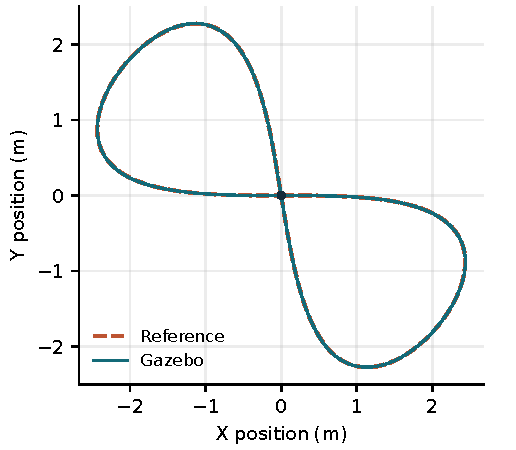
\includegraphics[width=0.78\columnwidth]{figures/trajectory.pdf}
\caption{Reference and observed rear-axle pose in Gazebo. The point marks the start near the central crossing.}
\label{fig:trajectory}
\end{figure}

\begin{figure}[t]
\centering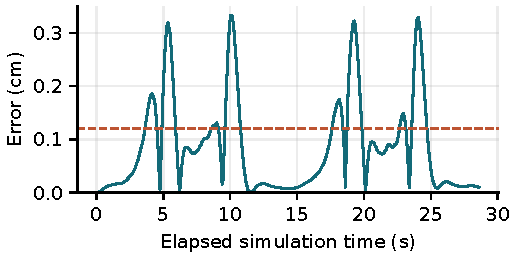
\includegraphics[width=0.81\columnwidth]{figures/tracking_error.pdf}
\caption{Path error versus elapsed simulation time. The dashed line marks the RMS error.}
\label{fig:error}
\end{figure}

The tracker completed the lap in \RunDuration\ s (\RunSamples\ samples) and commanded a stop at station \RunProgress\ m, \RunFinal\ cm from the endpoint. The RMS and peak path errors were \RunRMSE\ cm and \RunMax\ cm, respectively (Figs.~\ref{fig:trajectory} and~\ref{fig:error}). This trial used direct simulator pose and simplified contact geometry.

\section{Conclusion}
The controller completed the curvature-constrained figure eight and kept the intended branch at the intersection. Future trials should vary speed and lookahead, calibrate tire contact, and test localization based on encoders and an IMU.

\begin{thebibliography}{9}
\bibitem{lynch} K. M. Lynch and F. C. Park, \emph{Modern Robotics: Mechanics, Planning, and Control}. Cambridge University Press, 2017, ch.~13.
\bibitem{coulter} R. C. Coulter, \emph{Implementation of the Pure Pursuit Path Tracking Algorithm}. Carnegie Mellon University, Pittsburgh, PA, USA, Tech. Rep. CMU-RI-TR-92-01, 1992.
\bibitem{gzsource} Open Robotics, \emph{AckermannSteering system, Gazebo Sim 8}. \href{https://gazebosim.org/api/sim/8/classgz_1_1sim_1_1systems_1_1AckermannSteering.html}{Gazebo Sim API documentation}.
\bibitem{bridge} Open Robotics, \emph{Use ROS 2 to interact with Gazebo}. \href{https://gazebosim.org/docs/harmonic/ros2_integration/}{Gazebo Harmonic documentation}.
\end{thebibliography}
\end{document}
